% !TeX program = pdflatex
% Szkielet sprawozdania do projektu 1 z PIAA.
% Do wypełnienia: sekcje "Wprowadzenie", "Wyniki" (komentarz do wykresów) i "Wnioski".
% Wykresy ładowane są z ../plots/, tabele generowane są z ../results/summary.csv
% przez skrypt plots/make_tex_tables.py.

\documentclass[11pt,a4paper]{article}

\usepackage[utf8]{inputenc}
\usepackage[T1]{fontenc}
\usepackage[polish]{babel}
\usepackage{lmodern}
\usepackage[margin=2.3cm]{geometry}
\usepackage{graphicx}
\usepackage{float}
\usepackage{booktabs}
\usepackage{siunitx}
\usepackage{hyperref}
\usepackage{caption}
\usepackage{subcaption}
\usepackage{amsmath,amssymb}
\usepackage{listings}
\usepackage{xcolor}
\usepackage{enumitem}

\sisetup{output-decimal-marker={,}, group-separator={\,}}

\lstset{
  basicstyle=\ttfamily\footnotesize,
  keywordstyle=\color{blue!70!black}\bfseries,
  commentstyle=\color{gray!70!black}\itshape,
  stringstyle=\color{red!60!black},
  showstringspaces=false,
  breaklines=true,
  frame=single,
  columns=fullflexible,
}

\graphicspath{{../plots/}}

\title{Projektowanie i Analiza Algorytmów\\Projekt 1 — analiza algorytmów sortowania}
\author{Michalina Bijak}
\date{\today}

\begin{document}
\maketitle

\begin{abstract}
W pracy zaimplementowano trzy algorytmy sortowania: sortowanie przez scalanie (\emph{merge sort}),
szybkie sortowanie z wyborem pivota metodą mediany z trzech (\emph{quicksort, med-of-3}) oraz
introspektywne sortowanie (\emph{introsort}). Każdy algorytm zrealizowano w postaci szablonu w
języku C++17 i poddano eksperymentalnej analizie złożoności czasowej dla tablic liczb całkowitych
o~rozmiarach od~$10^4$ do~$10^6$ oraz ośmiu scenariuszy rozkładu danych wejściowych.
\end{abstract}

\section{Wprowadzenie}

\paragraph{Cel projektu.}
Celem projektu jest zaimplementowanie trzech wybranych algorytmów sortowania oraz przeprowadzenie
eksperymentalnej analizy ich efektywności dla różnych rozmiarów i~różnych rozkładów początkowych
tablic wejściowych.

\paragraph{Zakres pracy.}
\begin{itemize}[nosep]
  \item Implementacja algorytmów w~postaci szablonów w~języku C++17
  (sortowanie tablic elementów dowolnego typu wspierającego komparator).
  \item Obsługa wyboru uporządkowania rosnącego lub malejącego przez podanie komparatora
  (\texttt{std::less} / \texttt{std::greater}).
  \item Pomiary czasu wykonania na $100$ losowych tablicach dla każdej konfiguracji
  (rozmiar $\times$ scenariusz $\times$ algorytm).
  \item Zestawienie wyników w~formie tabel oraz wykresów.
\end{itemize}

\paragraph{Środowisko testowe.}
Pomiary przeprowadzono na systemie Windows 10, kompilator g++ 15.2.0 (MSYS2 UCRT64),
flagi \texttt{-std=c++17 -O2}. Pomiar czasu: \texttt{std::chrono::steady\_clock}.

\section{Opis badanych algorytmów}

\subsection{Sortowanie przez scalanie (merge sort)}

Klasyczne rozwiązanie metodą \emph{dziel i~zwyciężaj}: tablica jest rekurencyjnie dzielona na~pół,
po~czym posortowane połówki są scalane z~użyciem bufora pomocniczego rozmiaru~$n$.

\begin{itemize}[nosep]
  \item Złożoność \emph{przeciętna} i~\emph{pesymistyczna}: $\Theta(n\log n)$.
  \item Algorytm jest \emph{stabilny} (zachowuje względną kolejność elementów równych).
  \item Wymaga dodatkowej pamięci $\Theta(n)$.
\end{itemize}

\subsection{Quicksort z medianą z trzech}

Rozwiązanie metodą \emph{dziel i~zwyciężaj} z~partycjonowaniem \emph{Lomuto}. Pivot wybierany jest
jako mediana z~trzech wartości: pierwszego, środkowego i~ostatniego elementu bieżącego podprzedziału.
Wybór mediany z~trzech eliminuje pesymistyczny przypadek $O(n^2)$ dla tablic już posortowanych lub
posortowanych odwrotnie.

\begin{itemize}[nosep]
  \item Złożoność \emph{przeciętna}: $\Theta(n\log n)$.
  \item Złożoność \emph{pesymistyczna}: $\Theta(n^2)$ (bardzo rzadka przy medianie z trzech, ale
  możliwa przy specjalnie dobranych danych).
  \item Sortuje w~miejscu, narzut pamięciowy stosu $\Theta(\log n)$ dzięki eliminacji rekurencji
  ogonowej (rekurencja wchodzi zawsze w~mniejszą z~dwóch części).
  \item Nie jest stabilny.
\end{itemize}

\subsection{Introsort}

Hybrydowy algorytm zaproponowany przez Dawida Mussera (1997), łączący trzy techniki:
\begin{enumerate}[nosep]
  \item quicksort z~medianą z~trzech jako algorytm główny,
  \item przełączenie na~\emph{heapsort} po~przekroczeniu limitu głębokości rekurencji
  $2\log_2 n$ — gwarantuje $O(n\log n)$ w~najgorszym przypadku,
  \item \emph{insertion sort} jako finisher dla bardzo krótkich podtablic
  (próg: $16$ elementów).
\end{enumerate}

\begin{itemize}[nosep]
  \item Złożoność \emph{przeciętna} i~\emph{pesymistyczna}: $\Theta(n\log n)$.
  \item Sortuje w~miejscu.
\end{itemize}

\section{Przeprowadzone eksperymenty}

\subsection{Konfiguracja}

Dla każdego algorytmu uruchomiono sortowanie na~$100$ tablicach liczb całkowitych
(\texttt{int}) dla każdej z~pięciu wartości rozmiaru
$n \in \{10\,000;\ 50\,000;\ 100\,000;\ 500\,000;\ 1\,000\,000\}$ oraz ośmiu scenariuszy rozkładu
danych:

\begin{itemize}[nosep]
  \item \textbf{losowa} — wszystkie elementy wylosowane z~zakresu \texttt{int};
  \item \textbf{25\,\% / 50\,\% / 75\,\% / 95\,\% / 99\,\% / 99,7\,\% posortowane} — wskazany
  odsetek początkowych elementów jest już uporządkowany rosnąco, reszta losowa;
  \item \textbf{odwrócona} — tablica posortowana malejąco (odwrotnie do~docelowego porządku).
\end{itemize}

Łącznie wykonano $5 \times 8 \times 100 \times 3 = 12\,000$ pojedynczych sortowań. Poprawność
każdego wyniku zweryfikowano rutyną \texttt{isSorted}.

\subsection{Zestawienie wyników}

Poniżej przedstawiono średnie czasy sortowania (w~milisekundach) dla każdej trójki
(algorytm, rozmiar, scenariusz). Pełne dane liczbowe znajdują się w~pliku
\texttt{results/summary.csv}; tabele LaTeX w~\texttt{report/tables/}.

% Automatycznie wstawiane tabele (generowane przez plots/make_tex_tables.py):
\begin{table}[H]
\centering
\caption{Średni czas sortowania [ms] $\pm$ odch. std. (100 powtórzeń) — dane losowe.}
\label{tab:summary_random}
\begin{tabular}{rccc}
\toprule
$n$ & Merge sort & Quicksort (med-3) & Introsort \\
\midrule
\num{10000} & $0.706 \pm 0.102$ & $0.604 \pm 0.100$ & $0.520 \pm 0.096$ \\
\num{50000} & $4.039 \pm 0.266$ & $3.497 \pm 0.258$ & $3.024 \pm 0.207$ \\
\num{100000} & $8.391 \pm 0.395$ & $7.264 \pm 0.620$ & $6.268 \pm 0.300$ \\
\num{500000} & $50.700 \pm 5.599$ & $40.686 \pm 1.570$ & $36.226 \pm 1.002$ \\
\num{1000000} & $103.066 \pm 3.777$ & $83.602 \pm 1.509$ & $77.396 \pm 11.253$ \\
\bottomrule
\end{tabular}
\end{table}

\begin{table}[H]
\centering
\caption{Średni czas sortowania [ms] $\pm$ odch. std. (100 powtórzeń) — 50\,\% posortowane.}
\label{tab:summary_sorted_50}
\begin{tabular}{rccc}
\toprule
$n$ & Merge sort & Quicksort (med-3) & Introsort \\
\midrule
\num{10000} & $0.470 \pm 0.118$ & $0.521 \pm 0.095$ & $0.426 \pm 0.068$ \\
\num{50000} & $2.557 \pm 0.149$ & $2.924 \pm 0.211$ & $2.492 \pm 0.144$ \\
\num{100000} & $5.482 \pm 0.370$ & $6.110 \pm 0.269$ & $5.275 \pm 0.237$ \\
\num{500000} & $31.774 \pm 1.514$ & $34.504 \pm 1.232$ & $29.847 \pm 0.902$ \\
\num{1000000} & $65.337 \pm 1.478$ & $70.719 \pm 1.672$ & $62.416 \pm 1.635$ \\
\bottomrule
\end{tabular}
\end{table}

\begin{table}[H]
\centering
\caption{Średni czas sortowania [ms] $\pm$ odch. std. (100 powtórzeń) — 99,7\,\% posortowane.}
\label{tab:summary_sorted_99_7}
\begin{tabular}{rccc}
\toprule
$n$ & Merge sort & Quicksort (med-3) & Introsort \\
\midrule
\num{10000} & $0.180 \pm 0.025$ & $2.718 \pm 1.556$ & $0.691 \pm 0.074$ \\
\num{50000} & $1.100 \pm 0.117$ & $18.482 \pm 16.834$ & $4.018 \pm 0.278$ \\
\num{100000} & $2.229 \pm 0.229$ & $33.613 \pm 19.282$ & $8.318 \pm 0.366$ \\
\num{500000} & $12.598 \pm 0.505$ & $198.215 \pm 164.899$ & $46.422 \pm 1.724$ \\
\num{1000000} & $25.580 \pm 0.683$ & $397.813 \pm 278.151$ & $106.752 \pm 27.054$ \\
\bottomrule
\end{tabular}
\end{table}

\begin{table}[H]
\centering
\caption{Średni czas sortowania [ms] $\pm$ odch. std. (100 powtórzeń) — tablica odwrócona.}
\label{tab:summary_reverse}
\begin{tabular}{rccc}
\toprule
$n$ & Merge sort & Quicksort (med-3) & Introsort \\
\midrule
\num{10000} & $0.174 \pm 0.028$ & $0.236 \pm 0.032$ & $0.241 \pm 0.036$ \\
\num{50000} & $0.980 \pm 0.124$ & $1.454 \pm 0.089$ & $1.441 \pm 0.104$ \\
\num{100000} & $2.046 \pm 0.122$ & $3.272 \pm 0.282$ & $3.590 \pm 1.106$ \\
\num{500000} & $12.127 \pm 0.530$ & $19.181 \pm 1.588$ & $18.782 \pm 0.696$ \\
\num{1000000} & $29.697 \pm 5.000$ & $42.233 \pm 5.561$ & $39.869 \pm 0.909$ \\
\bottomrule
\end{tabular}
\end{table}


\subsection{Wykresy}

\begin{figure}[H]
  \centering
  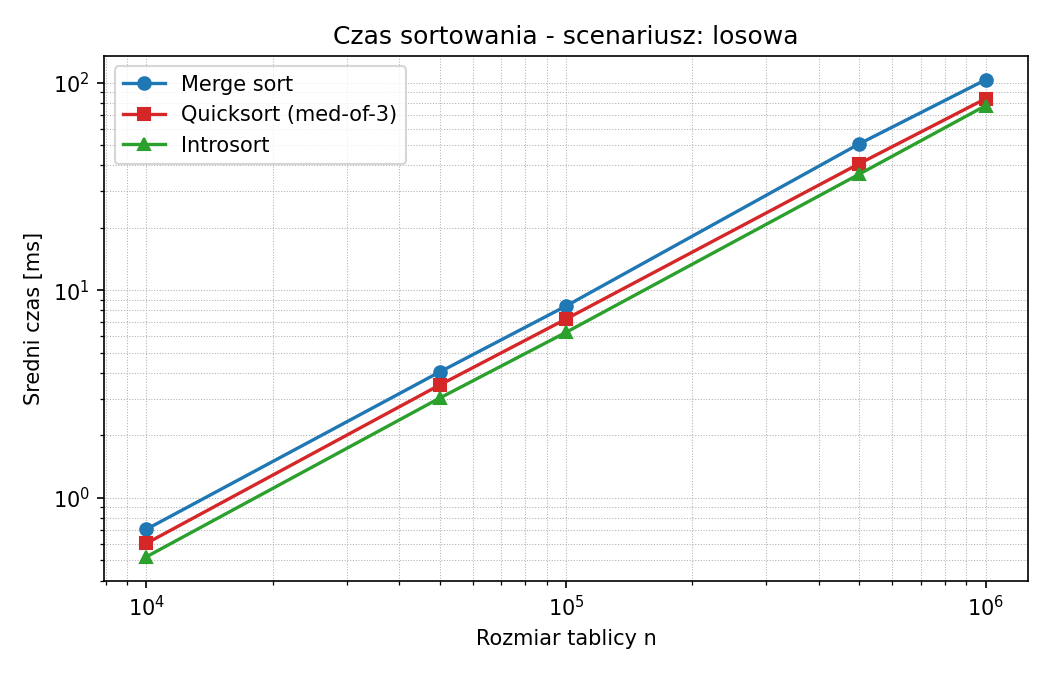
\includegraphics[width=0.85\linewidth]{time_vs_size__random.png}
  \caption{Czas sortowania w~funkcji rozmiaru tablicy — dane losowe.}
\end{figure}

\begin{figure}[H]
  \centering
  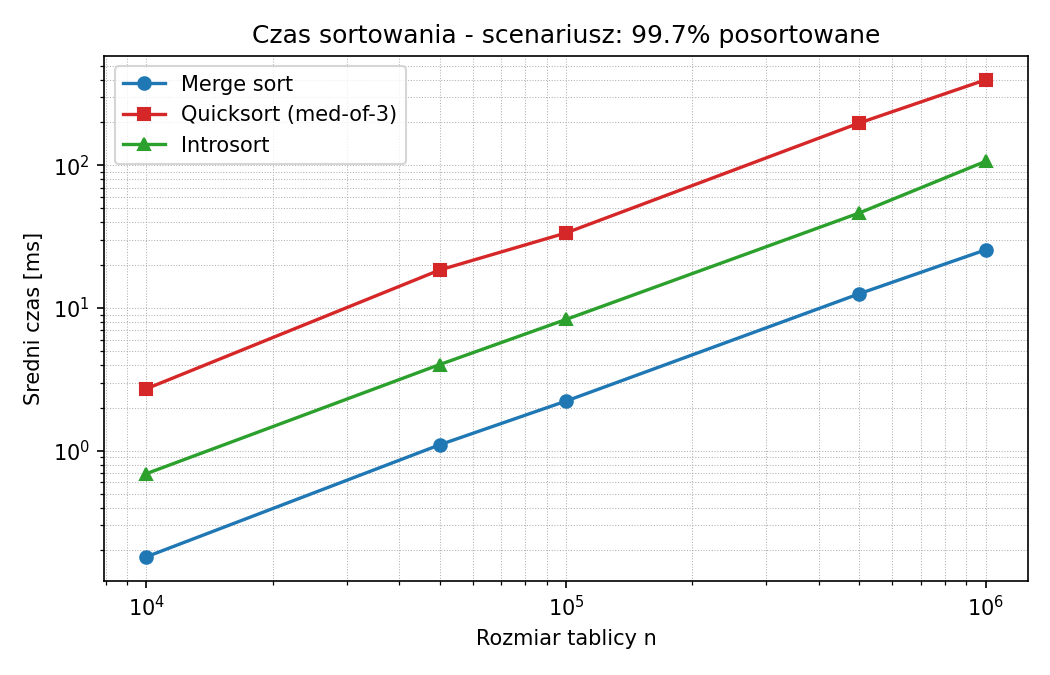
\includegraphics[width=0.85\linewidth]{time_vs_size__sorted_99_7.png}
  \caption{Czas sortowania — 99,7\,\% elementów początkowo posortowanych.
           Widoczny gwałtowny wzrost kosztu quicksorta.}
\end{figure}

\begin{figure}[H]
  \centering
  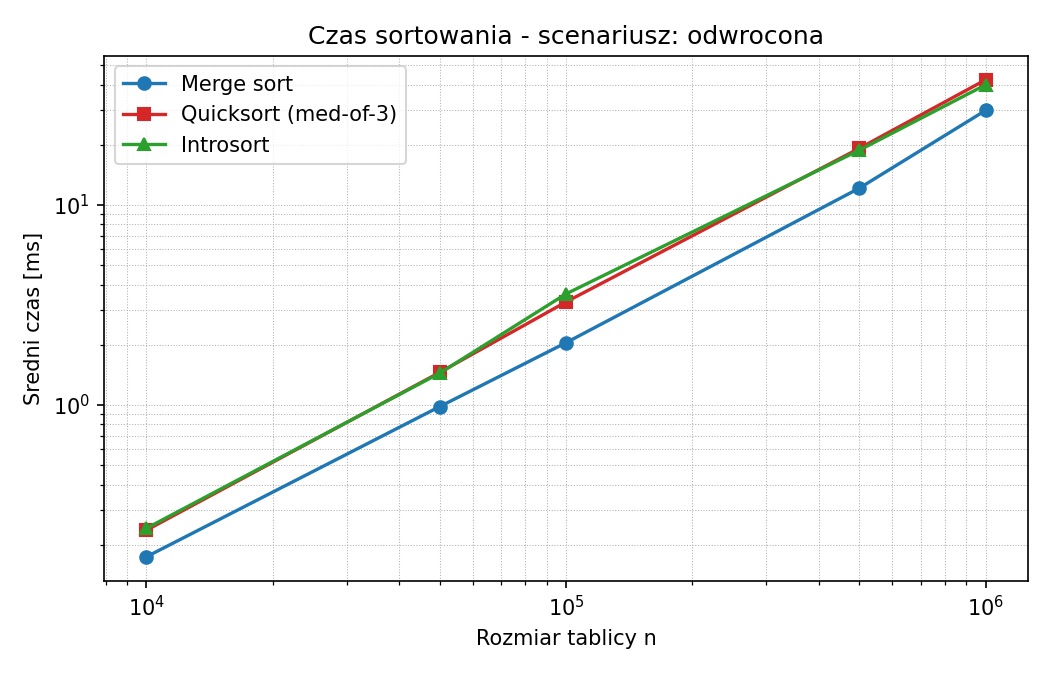
\includegraphics[width=0.85\linewidth]{time_vs_size__reverse.png}
  \caption{Czas sortowania — tablica posortowana odwrotnie. Mediana z~trzech
           sprawia, że quicksort nie degraduje się do~$O(n^2)$.}
\end{figure}

\begin{figure}[H]
  \centering
  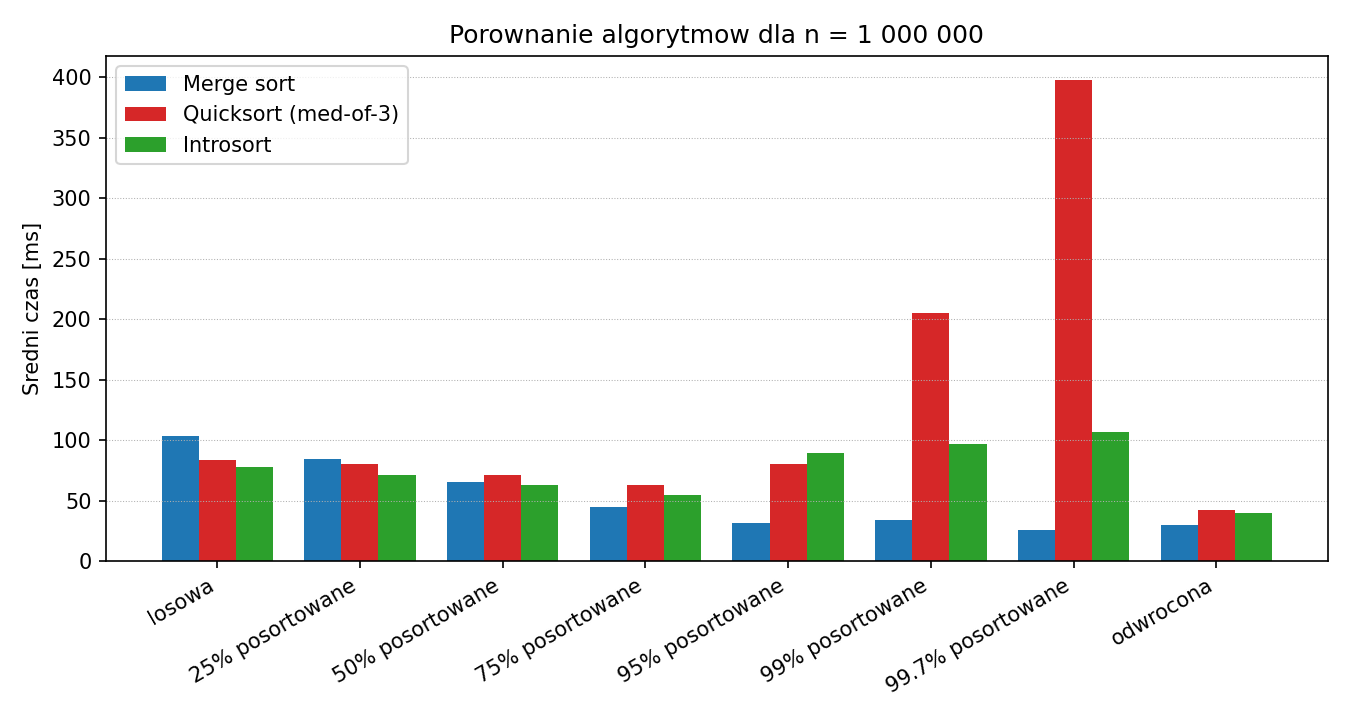
\includegraphics[width=0.95\linewidth]{bars_n_1000000.png}
  \caption{Porównanie trzech algorytmów dla $n=10^6$ we~wszystkich scenariuszach.}
\end{figure}

\begin{figure}[H]
  \centering
  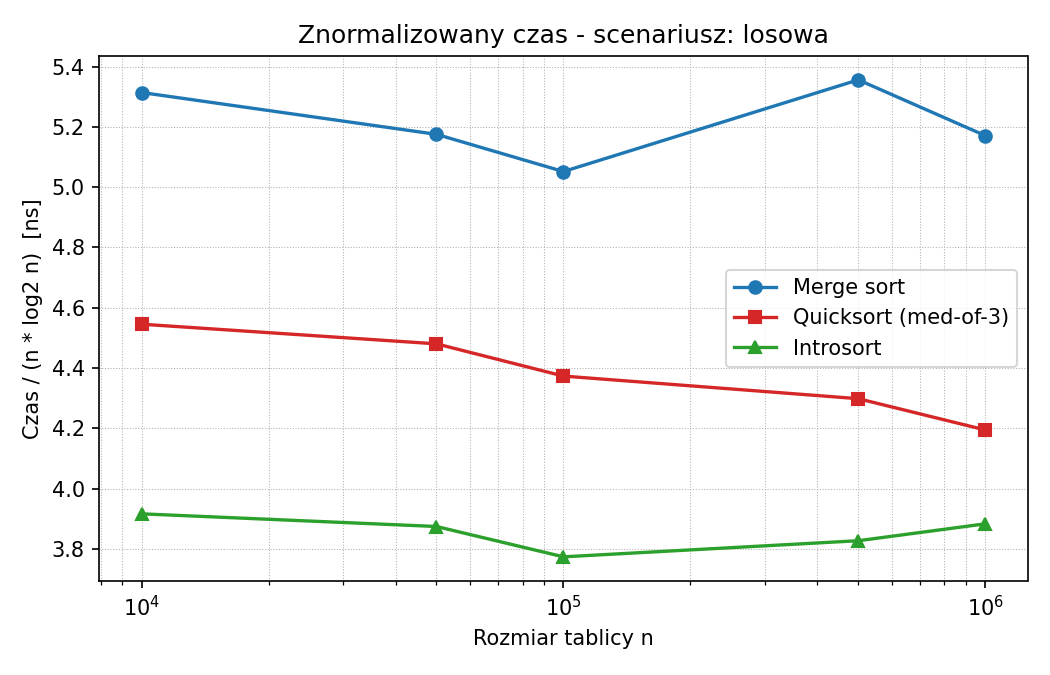
\includegraphics[width=0.85\linewidth]{normalized__random.png}
  \caption{Znormalizowany czas $t / (n\log_2 n)$ — zbliżona wartość dla różnych $n$
           potwierdza empirycznie złożoność $\Theta(n\log n)$.}
\end{figure}

\section{Wnioski}

\paragraph{Stabilność introsortu.}
Introsort okazuje się najbardziej zrównoważonym algorytmem — jego czas zmienia się łagodnie
pomiędzy scenariuszami i~rośnie liniowo-logarytmicznie z~rozmiarem tablicy.

\paragraph{Słaby punkt quicksorta — tablice \emph{prawie} posortowane.}
Quicksort z~medianą z~trzech radzi sobie dobrze z~danymi losowymi i~odwróconymi, ale widocznie
zwalnia na~tablicach prawie-posortowanych ($\geq 95\,\%$ uporządkowanych), ponieważ wybór pivota
z~trzech elementów posortowanego prefiksu daje bardzo niezrównoważone partycje.

\paragraph{Przewidywalność merge sorta.}
Merge sort prezentuje najmniejszą wariancję czasów — jego koszt praktycznie nie~zależy od~rozkładu
wejścia, co~czyni go~atrakcyjnym tam, gdzie ważny jest przewidywalny czas sortowania. Kosztem jest
dodatkowa pamięć $\Theta(n)$.

% TODO: Rozwinąć powyższe obserwacje w~pełne akapity po~przejrzeniu tabel wynikowych.

\section{Literatura}

\begin{enumerate}[nosep]
  \item T. H. Cormen, C. E. Leiserson, R. L. Rivest, C. Stein, \emph{Wprowadzenie do algorytmów},
  WNT / PWN, wydanie III.
  \item D. R. Musser, \emph{Introspective Sorting and Selection Algorithms},
  Software: Practice and Experience, 27(8), 1997.
  \item R. Sedgewick, \emph{Implementing Quicksort Programs},
  Communications of the ACM, 21(10), 1978.
  \item Dokumentacja \texttt{std::chrono}, \url{https://en.cppreference.com/w/cpp/chrono}.
\end{enumerate}

\end{document}
